\chapter{Marco teórico}

\section{Desde las ecuaciones de Maxwell a propagación de la luz en guías de onda dieléctricas}

Esta tesis estudia el comportamiento de luz láser de baja potencia (1 mW de potencia de salida) propagada en guías de onda dieléctricas escritas dentro de una muestra de borosilicato. Es por ello que se supone un medio lineal no magnético libre de fuentes de carga y de corriente. Las ecuaciones de Maxwell (SI) en este régimen son:
\begin{align}
	\nabla\cdot\textbf{D} &= 0, \label{eqn:gauss}
	\\	
	\nabla\times\textbf{E} &= -\frac{\partial \textbf{B}}{\partial t}, \label{eqn:faraday-lenz}
	\\	
	\nabla\cdot\textbf{B} &= 0,
	\\	
	\nabla\times\textbf{H} &= \frac{\partial \textbf{D}}{\partial t}, \label{eqn:ampere-maxwell}
\end{align}
donde \textbf{E}, \textbf{B}, $\textbf{D}=\varepsilon(\textbf{r})\textbf{E}$ y $\textbf{H}=\textbf{B}/\mu_0$ son los campos eléctrico, campo de densidad de flujo magnético, campo desplazamiento eléctrico y campo magnético, respectivamente. Las guías de onda son invariantes en la dirección de propagación $z$, por lo que el índice de refracción $n=\sqrt{\varepsilon/\varepsilon_0}$ dependerá de las coordenadas transversales al eje óptico, es decir, $n \equiv n(x,y) = n_0 + \Delta n(x,y)$, con $n_0=1.47$ el índice de refracción del borosilicato y $\Delta n \sim 10^{-5}-10^{-3}$ el contraste de las guías de onda.

Aplicando rotor por la izquierda a la ecuación de Faraday-Lenz (\ref{eqn:faraday-lenz}), usando la ecuación de Ampère-Maxwell (\ref{eqn:ampere-maxwell}) y asumiendo una solución temporal harmónica proporcional a $e^{-i\omega t}$ se tiene:

\begin{align}
	\nabla\times\nabla\times\textbf{E} &= -\frac{\partial}{\partial t}(\nabla\times\textbf{B}) = -\frac{\partial}{\partial t}\left(\mu_0\frac{\partial \textbf{D}}{\partial t}\right) = -\frac{n^2}{c^2}\frac{\partial^2 \textbf{E}}{\partial t^2} = n^2k_0^2 \textbf{E}, \label{eqn:rotordoble}
\end{align}
donde $k_0 \equiv \omega/c$ es el número de onda en el vacío. Notemos que, por identidad de cálculo vectorial, se tiene que $\nabla\times\nabla\times\textbf{E} = \nabla(\nabla\cdot\textbf{E}) - \nabla^2\textbf{E}$, y usando la ley de Gauss (\ref{eqn:gauss}) se deduce que $\nabla\cdot \textbf{E} = -\nabla(n^2)\cdot\textbf{E}/n^2$.

Con esto, se obtiene una ecuación tipo Helmholtz 

\begin{equation}
	(\nabla^2  + k_0^2n^2)\textbf{E} = -\nabla\left(\textbf{E} \cdot \frac{\nabla n^2}{n^2}\right) \approx 0, \label{eqn:helmholz}
\end{equation}

donde el término de la derecha se desprecia usando la aproximación de guiaje débil, pues el contraste $\Delta n$ es pequeño. 

\section{Soluciones analíticas para guía de onda tipo losa o \textit{slab}}

El sistema más simple que se puede estudiar es una guía de onda tipo losa, cuya forma analítica para el constraste $n(x)$ es la siguiente, con $n_1 > n_0$:

\begin{equation*}
	n(x) = \left\{\begin{matrix}
	n_1 \quad |x| \le a
	\\
	n_0 \quad |x| > a
 	\end{matrix}\right.
\end{equation*}

\begin{figure}[H]
	\centering
	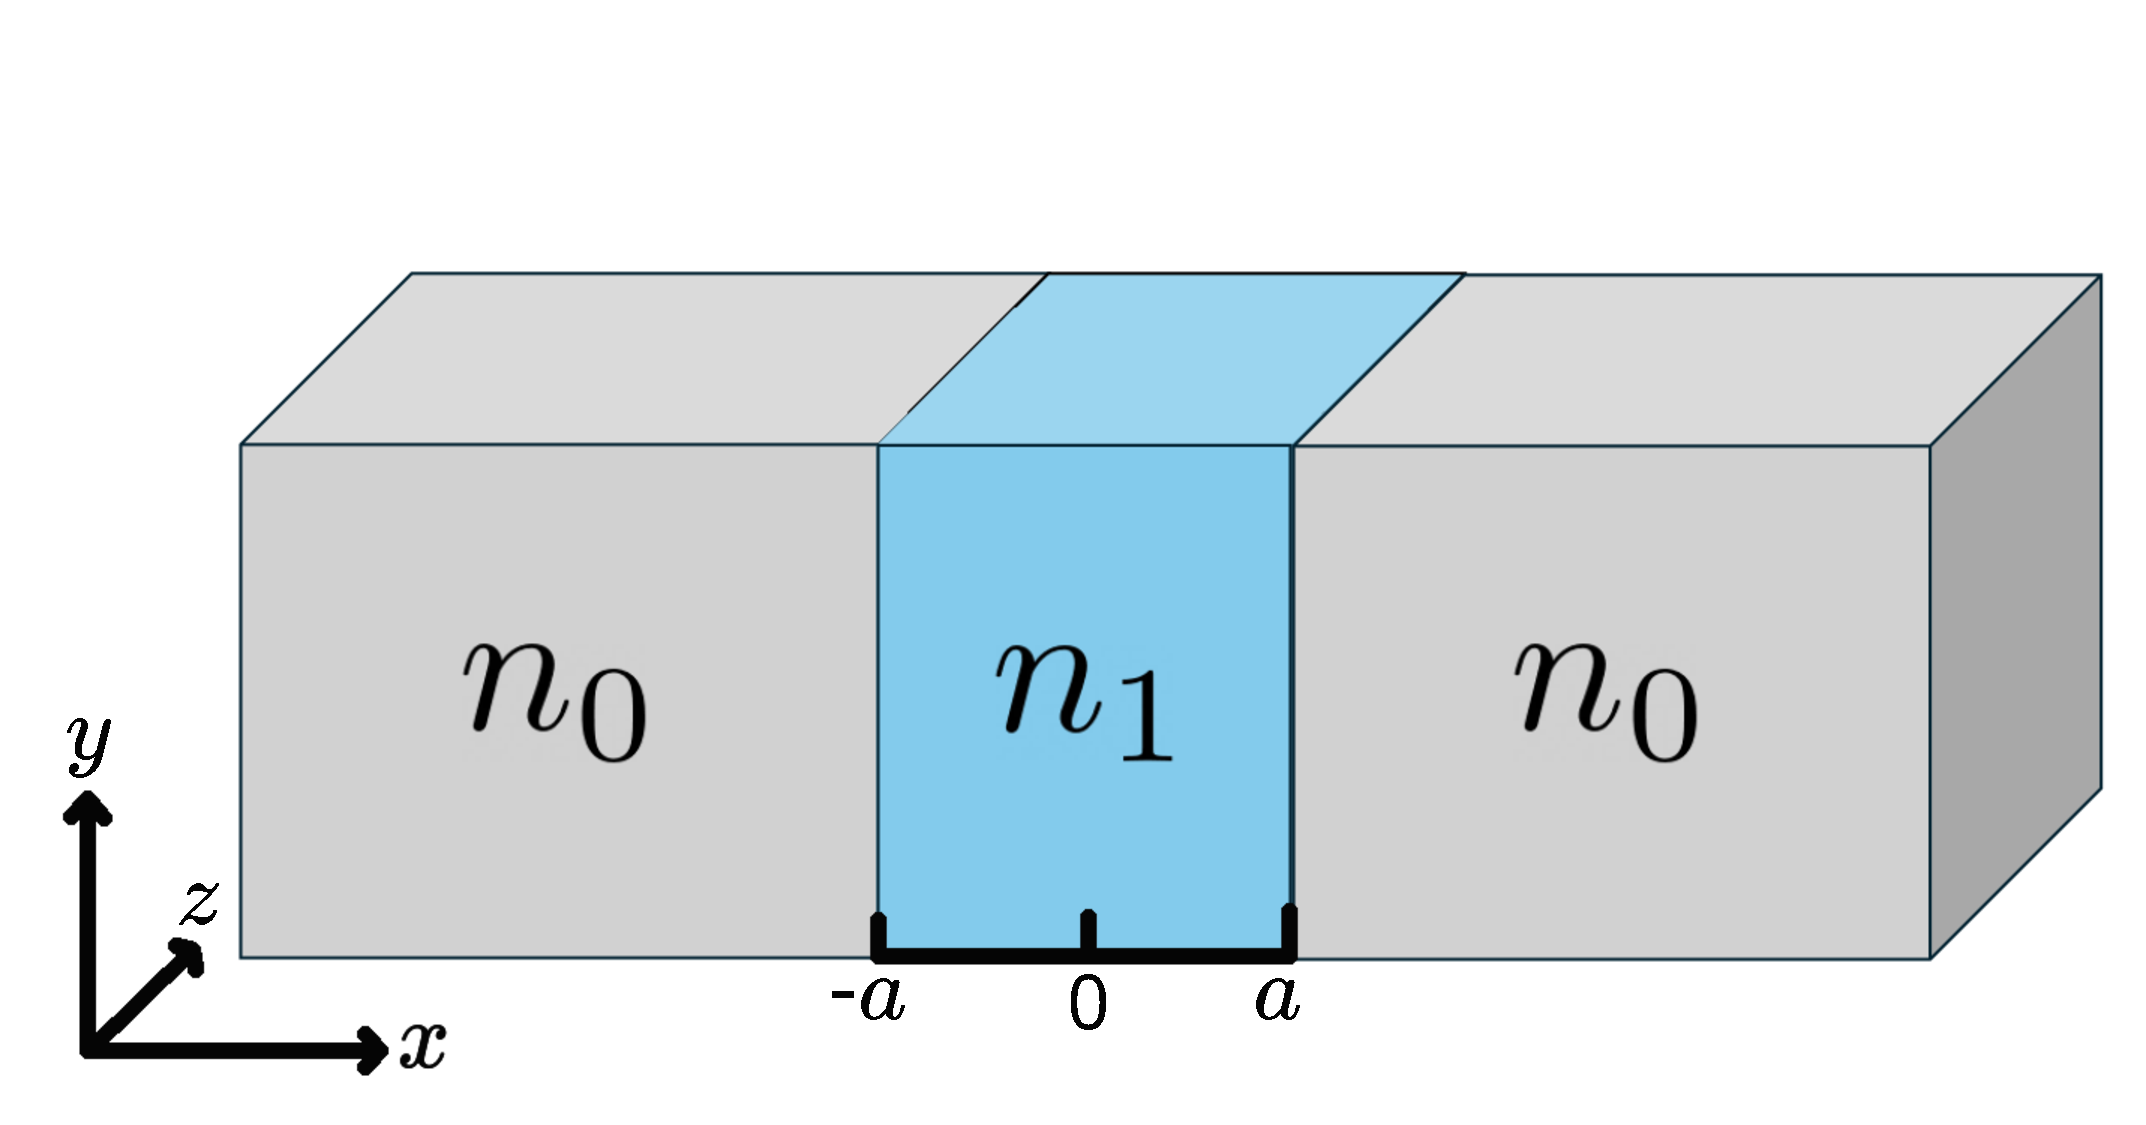
\includegraphics[width=0.6\linewidth]{media/slab.pdf}
	\caption[Forma de una guía de onda tipo losa.]{Forma de una guía de onda tipo losa. En las direcciones $\mathbf{\hat{y}}$ (vertical) y $\mathbf{\hat{z}}$ (hacia dentro de la página) la estructura es invariante.}
\end{figure}
\subsection{Modos TE}

Los modos transversales eléctricos o TE se expresan como $\textbf{E}(x,z) =\mathbf{\hat{y}} E_y= \mathbf{\hat{y}} E(x)e^{i k_z z }$, por lo que la ecuación (\ref{eqn:helmholz}) adquiere la forma

\begin{align}
(\nabla^2  + k_0^2n^2) E(x)e^{ik_z z} &=  \left(\frac{\partial^2}{\partial x^2} + \frac{\partial^2}{\partial z^2} + k_0^2n^2\right) E(x)e^{ik_z z } 
\nonumber
\\
&= e^{ik_z z}\left[\frac{d^2  E(x)}{dx^2}  + (k_0^2n^2 -  k_z^2)E(x) \right]
\nonumber
\\
&=0
\nonumber
\\
\therefore \frac{d^2  E(x)}{dx^2}  + (k_0^2n^2 -  k_z^2)E(x) &= 0 \label{eqn:TEslab}
\end{align}

Para encontrar soluciones cuya energía esté localizada en la guía de onda y que decaiga fuera de ella, se impondrá $k_0^2n_0^2 < k_z^2 < k_0^2n_1^2$. Se hace natural definir $\alpha^2\equiv k_0^2n_1^2-k_z^2$ y $\beta^2\equiv k_z^2 - k_0^2n_0^2$. \textcolor{red}{Incluir cita Griffiths QM acerca de soluciones pares e impares para potencial real simétrico}. Si consideramos soluciones pares, la ecuación (\ref{eqn:TEslab}) tendrá soluciones

\begin{equation*}
	E(x) = \left\{\begin{matrix}
	E_{s1}\cos(\alpha x)\quad |x|\le a
	\\
	E_{s0}e^{-\beta|x|} \quad |x|>a
	\end{matrix}\right.
\end{equation*}

Por otro lado, las soluciones impares tienen la forma
\begin{equation*}
	E(x) = \left\{\begin{matrix}
	E_{a1}\sin(\alpha x)\quad |x|\le a
	\\
	E_{a0}e^{-\beta|x|} \quad |x|>a
	\end{matrix}\right.
\end{equation*}


Es necesario considerar las condiciones de interfase electromagnéticas. En este caso, continuidad de las componentes de \textbf{E} y \textbf{H} paralelas a la interfaz . A partir de la ecuación de Faraday-Lenz (\ref{eqn:faraday-lenz}) se tiene:

\begin{align*}
	\nabla\times\textbf{E} &= -\mu_0\frac{\partial \textbf{H}}{\partial t}
	\\
	\mathbf{\hat{z}}\partial_x E_y-\mathbf{\hat{x}}\partial_z E_y  &= i\omega \mu_0  \textbf{H}
	\\	
	\therefore \textbf{H}_{||} = -i\mathbf{\hat{z}}\frac{e^{ik_z z}}{\omega\mu_0}\frac{d E(x)}{dx}.
\end{align*}
Es decir, tanto $E(x)$ como $\frac{dE(x)}{dx}$ deben ser continuos en $|x|=a$. Aplicando esto en $x=a$ separadamente para las soluciones simétricas y antisimétricas:

\begin{align*}
E_{s1}\cos(\alpha a) &= E_{s0} e^{-\beta a} & E_{a1}\sin(\alpha a) &= E_{a0} e^{-\beta a}
\\
E_{s1}\alpha\sin(\alpha a) &= \beta E_{s0} e^{-\beta a} & E_{a1}\alpha\cos(\alpha a) &= -\beta E_{a0} e^{-\beta a}
\end{align*}

Al dividir las ecuaciones de abajo por las de arriba se elimina la dependencia en las amplitudes y se obtienen ecuaciones trascendentales para $k_z$:

\begin{align}
	\alpha a \tan(\alpha a) &= \beta a, & \alpha a \cot(\alpha a) &= -\beta a \label{eqn:trascendentalTE}
\end{align}

Usando las dos ecuaciones (\ref{eqn:trascendentalTE}) junto a la restricción $(\alpha a)^2 + (\beta a)^2 = k_0^2 a^2(n_1^2 - n_0^2) \equiv V^2$ es posible obtener soluciones gráficas para las constantes de propagación $k_z$.

\begin{figure}[H]
	\centering
	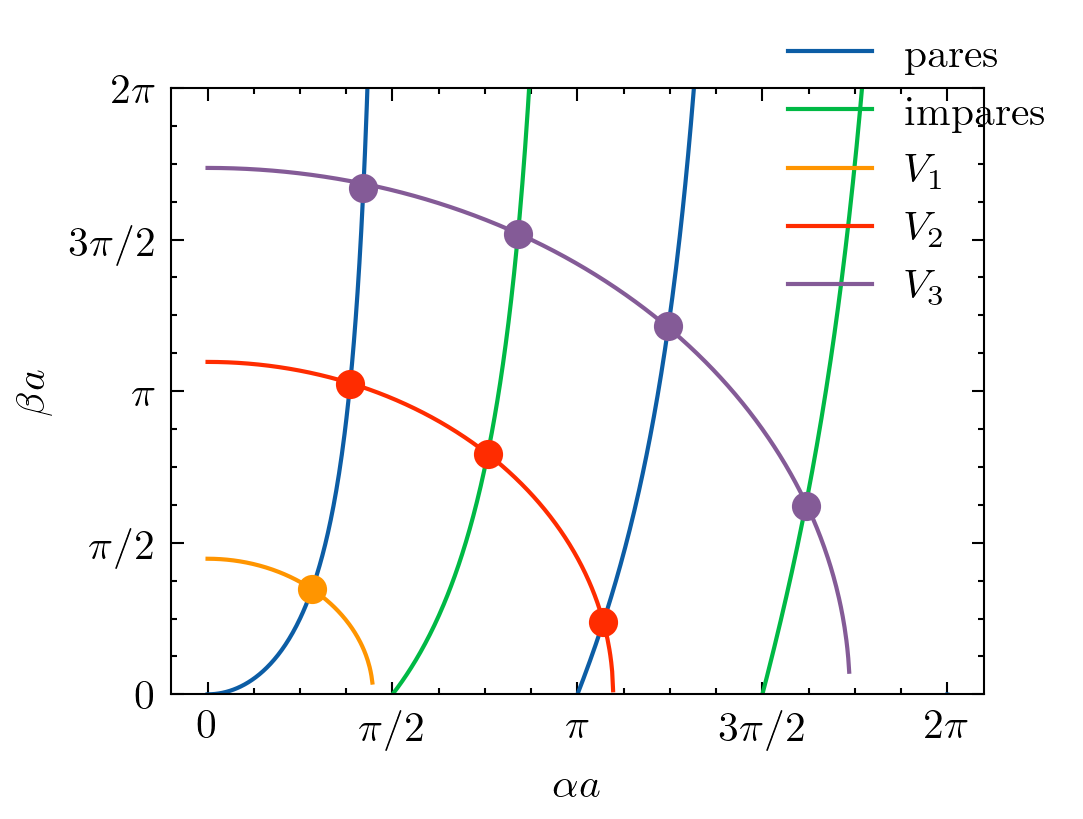
\includegraphics[width=0.7\linewidth]{media/slabgraphical}
	\caption[Soluciones gráficas de los modos TE]{Soluciones gráficas de los modos TE. A mayor contraste $\Delta n = n_1-n_0$, mayor cantidad de modos guiados soporta la guía de onda.}
\end{figure}
\subsection{Modos TM}
Los modos transversales magnéticos o TM se expresan como $\textbf{H}(x,z) =\mathbf{\hat{y}} H_y= \mathbf{\hat{y}} H(x)e^{i k_z z }$. Para expresar esta condición en términos del campo eléctrico $\textbf{E} = \textbf{E}_{||} + \textbf{E}_\perp$, se puede usar la ecuación de Ampère-Maxwell (\ref{eqn:ampere-maxwell}):

\begin{align*}
	\nabla\times\textbf{H} &= -\mathbf{\hat{x}} \partial_z H_y+ \mathbf{\hat{z}} \partial_x H_y = \mathbf{\hat{z}} e^{i k_z z }\frac{d H(x)}{dx} - \mathbf{\hat{x}} ik_z  e^{i k_z z } H(x)  
	\\	
	&= -i\omega\epsilon_0 n^2 \textbf{E}
	\\
	\therefore \textbf{E}_{||} = \mathbf{\hat{z}} \frac{ie^{i k_z z }}{n^2 \omega \epsilon_0} \frac{d H(x)}{dx}&,\quad \textbf{E}_\perp =  \mathbf{\hat{x}} \frac{k_z e^{i k_z z }}{n^2 \omega \epsilon_0 }   H(x).
\end{align*} 
Notemos que la ecuación (\ref{eqn:helmholz}) se puede separar por componentes, por lo que al considerar la ecuación que satisface la componente perpendicular $\textbf{E}_\perp$, se tiene:

\begin{align}
	(\nabla^2 + k_0^2 n^2) H_y
	&= \left(\frac{\partial^2}{\partial x^2} + \frac{\partial^2}{\partial z^2} + k_0^2n^2\right) H(x)e^{ik_z z }
	\nonumber
	\\
&= e^{ik_z z}\left[\frac{d^2  H(x)}{dx^2}  + (k_0^2n^2 -  k_z^2)H(x) \right]
\nonumber	
	\\	
	&= 0 
	\nonumber	
	\\
	\therefore 
	\frac{d^2  H(x)}{dx^2}  + (k_0^2n^2 -  k_z^2)H(x) &= 0
	\label{eqn:TMslab}
\end{align} 

La ecuación de modos TM (\ref{eqn:TMslab}) para $H(x)$ es idéntica que la ecuación (\ref{eqn:TEslab}) para $E(x)$ de modos TE. Es decir, definiendo $\alpha^2\equiv k_0^2n_1^2-k_z^2$ y $\beta^2\equiv k_z^2 - k_0^2n_0^2$ y considerando soluciones pares se tiene

\begin{equation*}
	H(x) = \left\{\begin{matrix}
	H_{s1}\cos(\alpha x)\quad |x|\le a
	\\
	H_{s0}e^{-\beta|x|} \quad |x|>a
	\end{matrix}\right.
\end{equation*}

Y las soluciones impares serán
\begin{equation*}
	H(x) = \left\{\begin{matrix}
	H_{a1}\sin(\alpha x)\quad |x|\le a
	\\
	H_{a0}e^{-\beta|x|} \quad |x|>a
	\end{matrix}\right.
\end{equation*}


Nuevamente, al considerar que $\textbf{H}_{||}= \mathbf{\hat{y}} H(x)e^{i k_z z }$ y $\textbf{E}_{||} = \mathbf{\hat{z}} \frac{ie^{i k_z z }}{n^2 \omega \epsilon_0} \frac{d H(x)}{dx}$ deben ser continuas, 

\begin{align*}
H_{s1}\cos(\alpha a) &= H_{s0} e^{-\beta a} & H_{a1}\sin(\alpha a) &= H_{a0} e^{-\beta a}
\\
H_{s1}\alpha\sin(\alpha a)/n_1^2 &= \beta H_{s0} e^{-\beta a}/n_0^2 & H_{a1}\alpha\cos(\alpha a)/n_1^2 &= -\beta H_{a0} e^{-\beta a}/n_0^2
\end{align*}

Al dividir las ecuaciones de abajo por las de arriba se elimina la dependencia en las amplitudes y se obtienen ecuaciones trascendentales implícitas en $k_z$:

\begin{align}
	\alpha a \tan(\alpha a)/n_1^2 &= \beta a/n_0^2, & \alpha a \cot(\alpha a)/n_1^2 &= -\beta a/n_0^2 \label{eqn:trascendentalTM}
\end{align}


\begin{figure}[H]
	\centering
	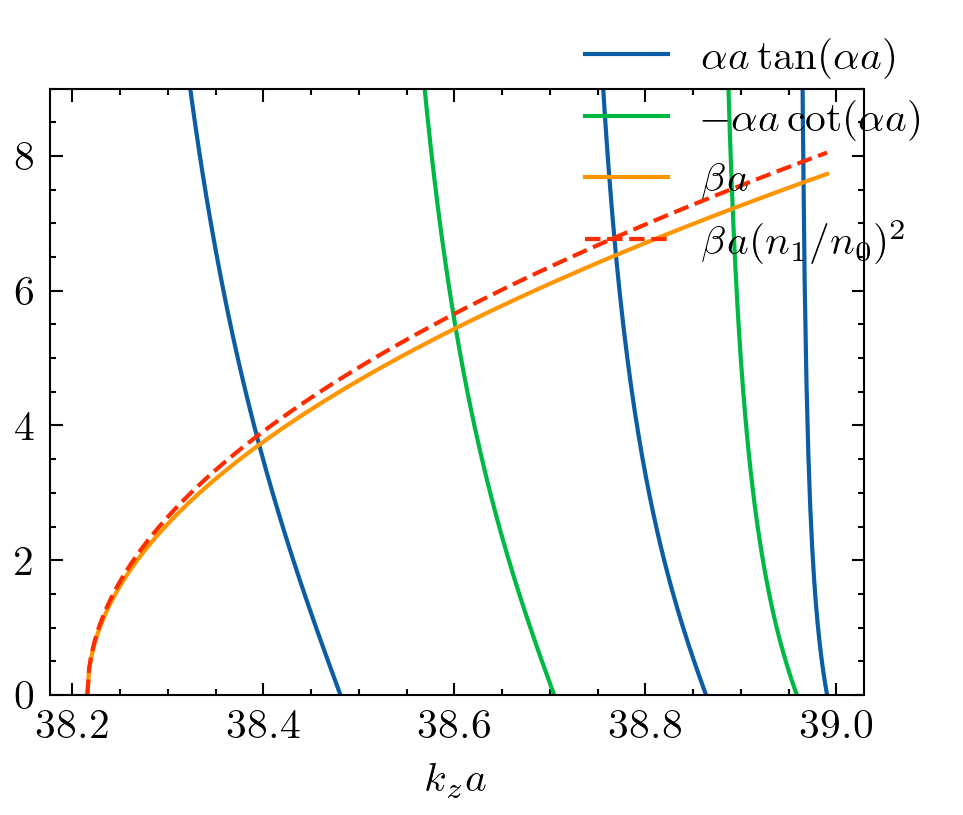
\includegraphics[width=0.7\linewidth]{media/slabgraphicalTETM1}
	\caption[Soluciones gráficas de los modos TE y TM]{Soluciones gráficas de los modos TE y TM para $\Delta n = 3\times 10^{-2}$. Se aprecia que las constantes de propagación de los modos TM son menores que las de los modos TE.}
\end{figure}
\section{Soluciones analíticas para fibra óptica circular}
En la sección anterior se estudió el sistema más sencillo en el que se puede hablar de guías de onda dieléctricas. El siguiente paso en complejidad consiste en guías de onda circulares. Para ello, se considerará que el índice de refracción varía radialmente según 

\begin{equation}
	n(r) = 
	\left\{\begin{matrix}
	n_1, \quad \text{si } \rho \le a
	\\
	n_0, \quad \text{si } \rho > a
	\end{matrix}\right.
	,\nonumber
\end{equation}
donde la tupla $(\rho, \phi, z)$ define las coordenadas cilíndricas a usar, más apropiadas para este problema. Al usar la separación de variables $ \textbf{E}(\textbf{r}) =  \textbf{E}_0 R(\rho)\Phi(\phi) e^{ik_z z} $ la ecuación (\ref{eqn:helmholz}) toma la forma:

\begin{align}
	\left[\frac{\partial^2}{\partial \rho^2} + \frac{\partial}{\rho\partial \rho} + \frac{\partial^2}{\rho^2\partial \phi^2} +\left( k_0^2n^2 - k_z^2 \right)\right]  R(\rho)\Phi(\phi) = 0
	\nonumber
	\\
\rho^2\frac{d^2 R}{Rd\rho^2} + \rho\frac{dR}{Rd\rho} + \rho^2\left( k_0^2n^2 - k_z^2 \right) + \underbrace{\frac{d^2 \Phi}{\Phi d\phi^2}}_{-\ell^2} = 0
\nonumber
\\
\therefore \Phi(\phi) = A\cos(\ell\phi) + B\sin(\ell\phi)
\nonumber
\end{align}
Imponiendo condiciones de periodicidad $\Phi(0)=\Phi(2\pi)$ y $\Phi'(0)=\Phi'(2\pi)$, se tiene que $B=A\tan(\pi \ell)$, luego $0 = \tan(\ell \pi)$. Es decir, $\ell$ debe ser un número entero y $\Phi(\phi) = A\cos(\ell\phi)$.

La ecuación para $R(\rho)$ es de tipo Bessel, por lo que definiendo $\alpha^2 \equiv k_0^2n_1^2 - k_z^2$ y $\beta^2\equiv k_z^2 - k_0^2n_0^2$ se tiene:

\begin{align}
	\frac{d^2 R}{d\rho^2} + \frac{1}{\rho}\frac{dR}{d\rho} + \left( k_0^2n^2 - k_z^2 -\frac{\ell^2}{\rho^2}\right)R  = 0
	\nonumber
	\\
	\therefore R(\rho) = 
	\left\{
	\begin{matrix}	
	C_1 J_\ell (\alpha\rho) + D_1 Y_\ell (\alpha\rho), \quad \text{si } \rho \le a  
	\\
	C_2 K_\ell (\beta\rho) + D_2 I_\ell (\beta\rho), \quad \text{si } \rho > a  
	\end{matrix}
	\right.
	. \nonumber
\end{align}
Necesariamente se debe imponer $D_1 = D_2 = 0$ para que la solución sea finita para $\rho = 0$ y para $\rho \to +\infty$. Es decir, la parte radial de la solución es
\begin{align*}
 R(\rho) = 
	\left\{
	\begin{matrix}	
	C_1 J_\ell (\alpha\rho), \quad \text{si } \rho \le a  
	\\
	C_2 K_\ell (\beta\rho), \quad \text{si } \rho > a  
	\end{matrix}
	\right.
	. \nonumber
\end{align*}
\subsection{Modos TE}
\subsection{Modos TM}
\section{Modos normales en guías de onda}

Si la estructura de guías de onda no varía en la dirección $z$, el campo eléctrico se puede expresar como una onda plana del tipo $\textbf{E}(\textbf{r}) = \textbf{E}_\nu(x, y) e^{i\beta_\nu z}$. A su vez, es conveniente separar el laplaciano como $\nabla^2 \equiv \nabla_\perp^2 + \frac{\partial^2}{\partial z^2}$. De esta forma la ecuación (\ref{eqn:helmholz}) se expande como:

\begin{align}
	(\nabla^2  + k_0^2n^2) \textbf{E}(\textbf{r}) &= \left(\nabla_\perp^2 + \frac{\partial^2}{\partial z^2} + k_0^2n^2\right) \textbf{E}_\nu(x, y)  e^{i\beta_\nu z} \nonumber
\\	
	&= e^{i\beta_\nu z} \nabla_\perp^2 \textbf{E}_\nu -\beta_\nu^2\textbf{E}_\nu e^{i\beta_\nu z} + k_0^2n^2 \textbf{E}_\nu  e^{i\beta_\nu z}
\nonumber	
	\\	
	&= \left[  \nabla_\perp^2  + (k_0^2n^2-\beta_\nu^2) \right]\textbf{E}_\nu  e^{i\beta_\nu z}
	\nonumber	
	\\
	&=
	0
	\nonumber
	\\
	\therefore
	 \left[  \nabla_\perp^2  + k_0^2n^2(x,y) \right]&\textbf{E}_\nu(x,y)  = \beta_\nu^2 \textbf{E}_\nu(x,y) \label{eqn:eigenfield}
\end{align}
Notemos que la ecuación (\ref{eqn:eigenfield}) es un problema de autovalores $\beta_\nu^2$ y autofunciones $\textbf{E}_\nu(x,y)$, que son ortogonales y forman una base completa (ver apéndice \ref{sec:orto}). En principio, la forma espacial del índice de refracción $n(x, y)$ puede ser arbitraria siempre y cuando que se satisfaga la condición de guiaje débil de la ecuación (\ref{eqn:helmholz}). 

\section{Teoría de modos acoplados}
	Para el estudio de redes fotónicas, es conveniente utilizar herramientas similares a las de la Física del Sólido en lo que respecta a potenciales periódicos. En particular, se puede suponer que los modos guiados de una guía de onda están fuertemente ligados a ella (enlace fuerte o \textit{Tight Binding}), incluso en presencia de otras guías de onda. Es decir, se supondrá que el $\nu$-ésimo modo de la $m$-ésima guía de onda satisface para toda distancia de propagación $z$ la ecuación (\ref{eqn:eigenfield}), donde el índice de refracción total se puede descomponer en una suma periódica de guías de onda $n^2(\textbf{r}) = \sum_{m} n^2_m(\textbf{r})$. Entonces, descomponiendo el campo eléctrico total de la forma $\textbf{E}(\textbf{r}) = \sum_{\nu, m} \textbf{E}_{\nu, m}(x, y) a_{\nu, m}(z) e^{i\beta_{\nu, m} z}$ y reemplazando en la ecuación (\ref{eqn:helmholz}) se tiene:

\begin{align}
	(\nabla^2  + k_0^2n^2) \textbf{E}(\textbf{r}) &= \left(\nabla_\perp^2 + \frac{\partial^2}{\partial z^2} + k_0^2n^2 \right)\sum_{\nu, m} \textbf{E}_{\nu, m}(x, y) a_{\nu, m}(z) e^{i\beta_{\nu, m} z}
	\nonumber
	\\
	&= \sum_{\nu, m} \left[a_{\nu, m} e^{i\beta_{\nu, m} z} \left(\nabla_\perp^2 +k_0^2n^2 \right)\textbf{E}_{\nu, m} + \textbf{E}_{\nu, m}\frac{d^2}{d z^2}\left(a_{\nu, m} e^{i\beta_{\nu, m} z}\right)\right]
	\nonumber	
	\\
	&= \sum_{\nu, m} \left[a_{\nu, m}  \left(\nabla_\perp^2 +k_0^2n^2 -\beta_{\nu,m}^2 \right) + \frac{d^2 a_{\nu, m}}{d z^2}  +2i\beta_{\nu,m}\frac{d a_{\nu, m}}{d z} \right]e^{i\beta_{\nu, m} z}\textbf{E}_{\nu, m}
		\nonumber	
	\\
	&\approx \sum_{\nu, m} \left[a_{\nu, m}  k_0^2(n^2 - n^2_{m}) +2i\beta_{\nu,m}\frac{d a_{\nu, m}}{d z} \right]e^{i\beta_{\nu, m} z}\textbf{E}_{\nu, m}
	\nonumber	
	\\
	&= 0,
	\nonumber	
\end{align}
Donde se ha usado que $\left|\frac{d^2 a_{\nu, m}}{d z^2}\right|\ll 2\beta_{\nu,m}\left|\frac{d a_{\nu, m}}{d z}\right|  $, conocida como aproximación paraxial. Aplicando producto punto con $\textbf{E}_{\mu, m'}^*$ e integrando en todo el plano $xy$:
\begin{align}
	  \int\displaylimits_{-\infty}^{+\infty}\int\displaylimits_{-\infty}^{+\infty} \sum_{\nu, m} \left[a_{\nu, m}  k_0^2(n^2 - n^2_{m}) +2i\beta_{\nu,m}\frac{d a_{\nu, m}}{d z} \right]e^{i\beta_{\nu, m} z}\textbf{E}_{\nu, m} \cdot \textbf{E}_{\mu, m'}^* dxdy &= 0
	  \nonumber
	  \\
	  \sum_{\nu, m} \left(2i\beta_{\nu,m}\frac{d a_{\nu, m}}{d z} \delta_{\nu,\mu}\delta_{m,m'} +  2\beta_{\mu, m'}C_{m', m, \nu, \mu}   a_{\nu, m} \right)e^{i\beta_{\nu, m} z} &= 0
	  \nonumber
	  \\
	  	  i\frac{d a_{\mu, m'}}{d z} e^{i\beta_{\mu, m'} z} +  \sum_{\nu, m\neq m'}C_{m', m, \nu, \mu}   a_{\nu, m} e^{i\beta_{\nu, m} z} &= 0
	\label{eqn:CMT1}
\end{align}
donde se han definido y usado
\begin{align*}
	   \int\displaylimits_{-\infty}^{+\infty}\int\displaylimits_{-\infty}^{+\infty} k_0^2(n^2 - n^2_{m}) \textbf{E}_{\nu, m} \cdot \textbf{E}_{\mu, m'}^* dxdy &\equiv 2\beta_{\mu, m'}C_{m', m, \nu, \mu}  
	\nonumber
	\\
	\int\displaylimits_{-\infty}^{+\infty}\int\displaylimits_{-\infty}^{+\infty} \textbf{E}_{\nu, m} \cdot \textbf{E}_{\mu, m'}^* dxdy &\approx \delta_{\nu,\mu}\delta_{m,m'}.
\end{align*}
Es decir, el efecto del modo $(\nu, m)$ en la dinámica del modo $(\mu, m')$ sólo es apreciable al ponderar con la expresión $(n^2 - n^2_{m})$, lo que da origen al término $C_{m', m, \nu, \mu}$ conocido comúnmente como constante de acoplamiento. Sin el peso del contraste, la interacción es evanescente, por lo que la aproximación de ortogonalidad se hace razonable con suficiente distancia entre guías (sobre los 15 $\mu$m en los experimentos de esta tesis). Cuando $m=m'$, el acoplamiento $C_{m', m, \nu, \mu}$ es nulo por definición. Es por ello que no se incluye en la sumatoria de la ecuación (\ref{eqn:CMT1}). 

Para fijar ideas, consideremos el caso del dímero monomodal homogéneo, considerando una distancia $d$ entre guías \textcolor{red}{INCLUIR ESQUEMA PARA EXPLICAR ACOPLAMIENTO}. El índice de refracción en este caso es $n^2 = n_1^2 + n_2^2$, con $n_1(\textbf{r})=n_2(\textbf{r}+\textbf{d})$. Dada la simetría del problema, la constante de acoplamiento se puede desarrollar como 
\begin{align}
	C_{1, 2} &=  \frac{1}{2\beta}\int\displaylimits_{-\infty}^{+\infty}\int\displaylimits_{-\infty}^{+\infty} k_0^2 n_1^2(\textbf{r}) \textbf{E}_{2}(\textbf{r}) \cdot \textbf{E}_{1}^*(\textbf{r}) dxdy 
	= \frac{k_0^2}{2\beta}\int\displaylimits_{-\infty}^{+\infty}\int\displaylimits_{-\infty}^{+\infty}  n_2^2(\textbf{r}+\textbf{d}) \textbf{E}_{1}(\textbf{r}+\textbf{d}) \cdot \textbf{E}_{1}^*(\textbf{r}) dxdy 
	\nonumber	
	\\	
	&= \frac{k_0^2}{2\beta}\int\displaylimits_{-\infty}^{+\infty}\int\displaylimits_{-\infty}^{+\infty} n_2^2(\textbf{r}) \textbf{E}_{1}(\textbf{r}) \cdot \textbf{E}_{1}^*(\textbf{r}-\textbf{d}) dxdy 
	= \frac{k_0^2}{2\beta}\int\displaylimits_{-\infty}^{+\infty}\int\displaylimits_{-\infty}^{+\infty} n_2^2(\textbf{r}) \textbf{E}_{1}(\textbf{r}) \cdot \textbf{E}_{2}^*(\textbf{r}) dxdy 
	\nonumber
	\\	
	&= C_{2,1} \equiv C
	\nonumber
\end{align}
 por lo que las dos ecuaciones dinámicas se escriben como:

\begin{equation}
	i\frac{d a_1}{dz} + C a_2 = 0, \quad\quad i\frac{d a_2}{dz} + C a_1 = 0 \nonumber
\end{equation}


	
